\chapter{Pairwise Comparison}\label{sec:compare}
\minitoc

\begin{sidewaysfigure}
\centering
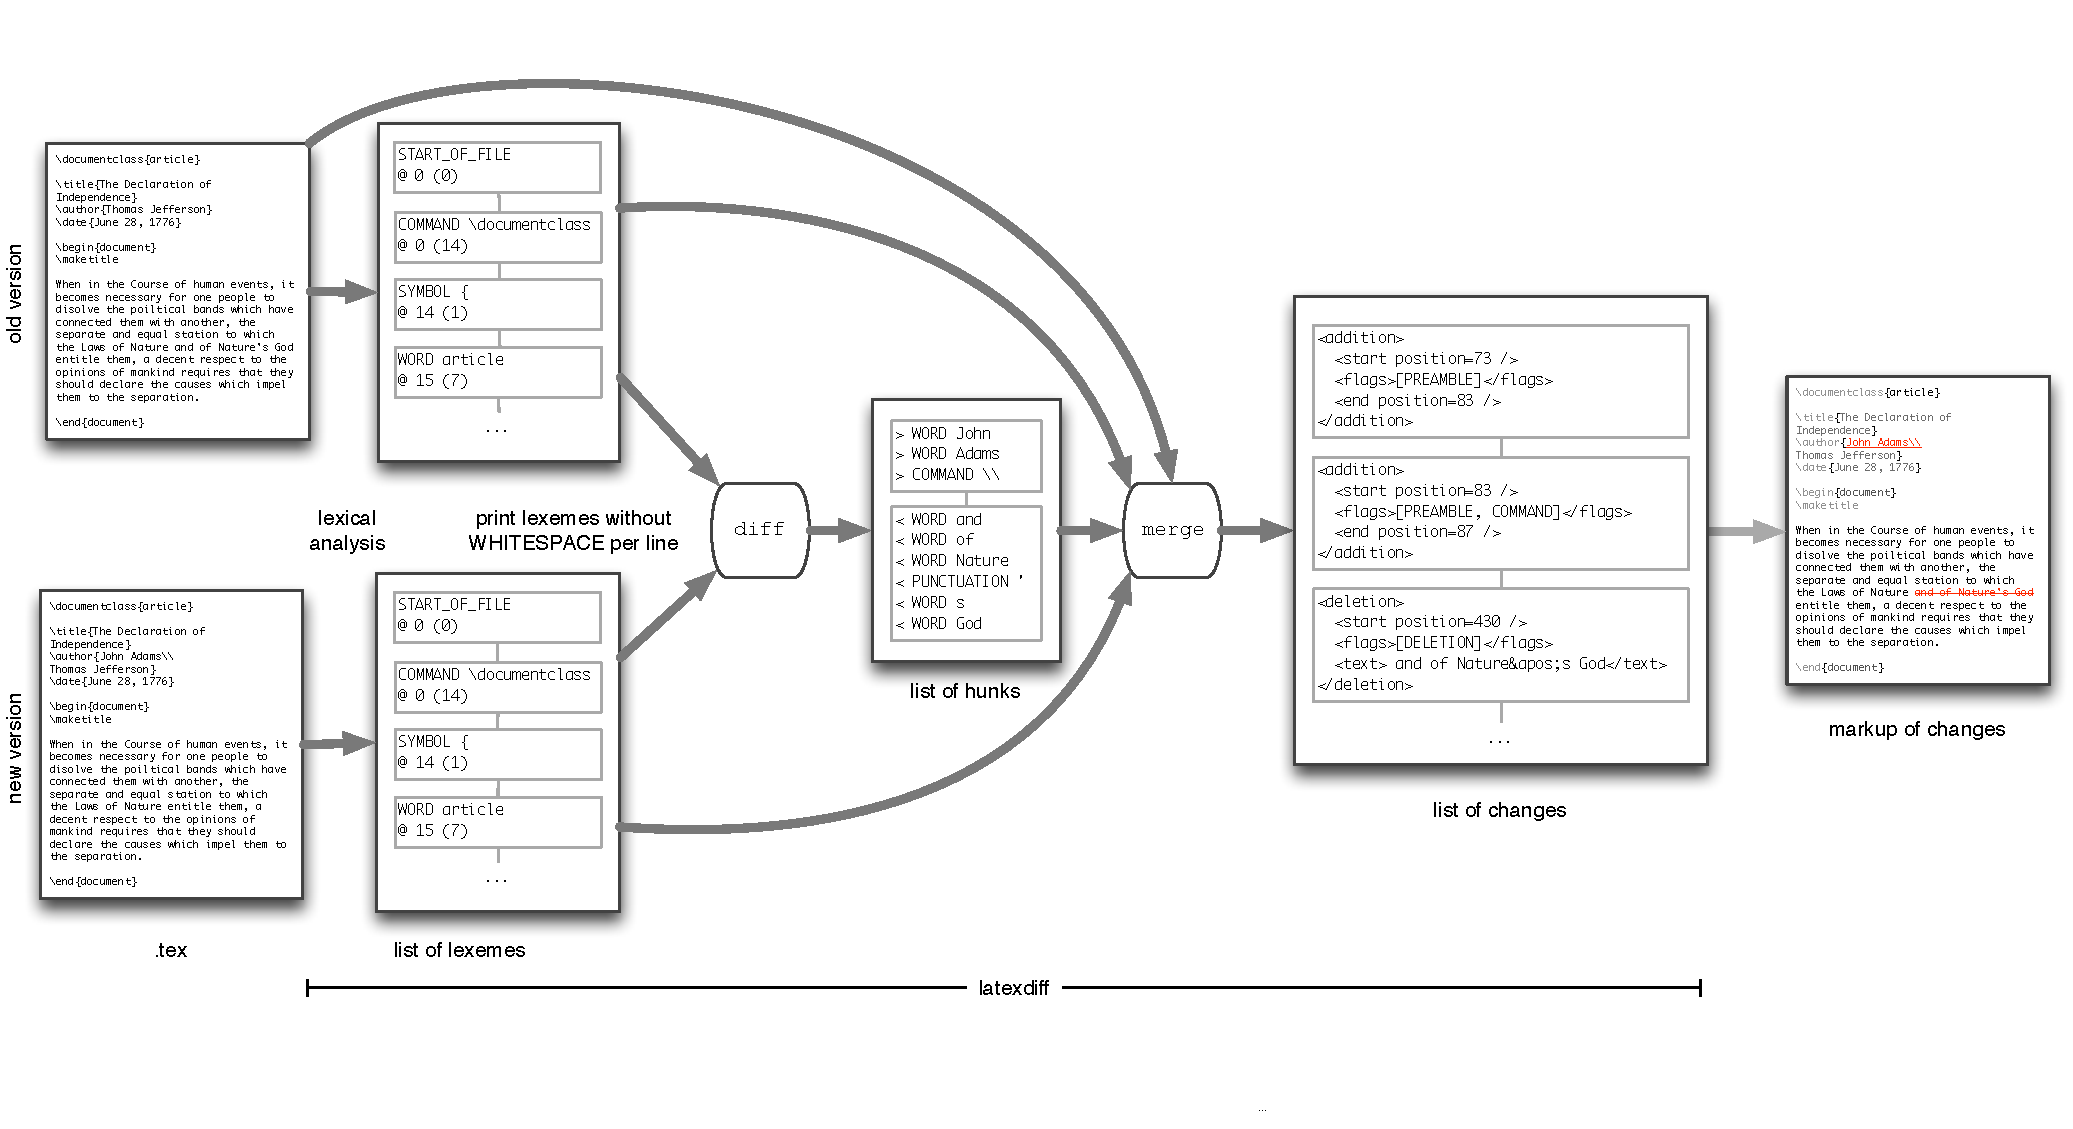
\includegraphics[width=\textwidth]{./figures/latexdiff3}
\caption{Example of performing \texttt{latexdiff} between two versions} \label{fig:latexdiff}
\end{sidewaysfigure}

In this chapter, we describe our LaTeX-aware diff algorithm called \texttt{latexdiff} that compares two LaTeX source files in a meaningful way.  In particular, \texttt{latexdiff} ignores changes in white space unless it creates or removes a paragraph delimiter\footnote{Note that our detection of paragraphs is an approximation: We define paragraph delimiters as two or more newline characters with possibly connecting other white space that occur after the preamble or everywhere in the file if no preamble exists. This definition does not take into account that paragraph space also exists after sectioning commands etc. even if there are less than two newline characters.  It would make our lexical analysis too complicated if we were to parse the LaTeX source files for more accurate detection of paragraph delimiters.} in the body of a LaTeX document. See Figure~\ref{fig:latexdiff} for an overview of \texttt{latexdiff}. 

The output of \texttt{latexdiff} contains additional information on top of the bare differences to aid marking up changes in a file.  For example, we need location information in order to locate changes in the newer version of the file, and flags for filtering certain changes to the viewer.

\section{Lexical Analysis}

Lexical analysis is the process of converting a sequence of characters into a sequence of tokens. Programs performing lexical analysis are called lexical analyzers or lexers.  

\begin{figure} 
\centering
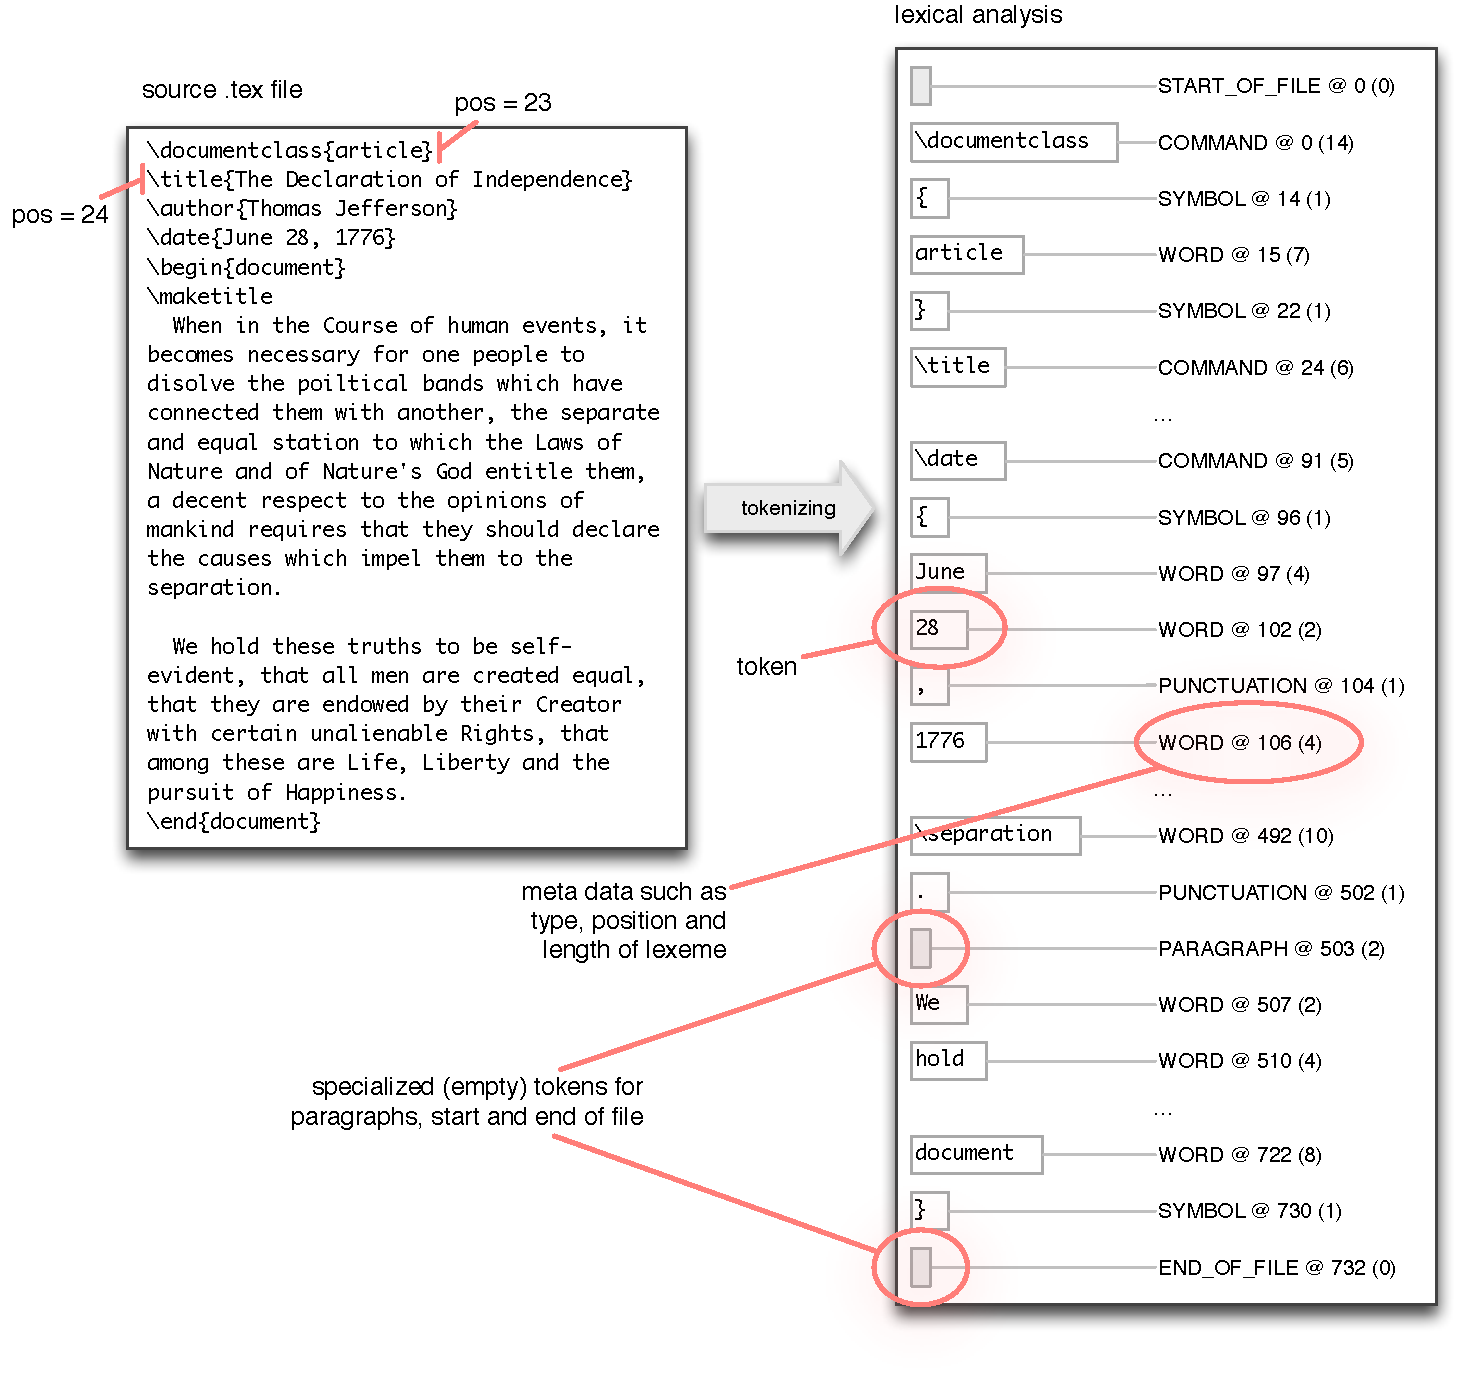
\includegraphics[width=0.9\textwidth]{./figures/tokenizer-example}
\caption{Example of tokenizing source text in preparation for diff'ing} \label{fig:tokenizer-example}
\end{figure}

\lstinputlisting[float,basicstyle=\tiny\ttfamily,
caption={Part of lexer.jflex to perform lexical analysis},label=lst:lexer.jflex,numbers=none,linerange={11-13,22-24,61-130}]{../../../../../ltc-server/src/main/jflex/lexer.jflex}

We call the tokens generated by lexical analysis ``lexemes'' and compare source files lexeme-by-lexeme.  A lexeme is a word, a LaTeX command, punctuation, symbols, non-whitespace parts of comments, or paragraph delimiters (see footnote above about the accuracy of detecting paragraph delimiters).  White space is ignored, however, we still need to keep track of location information in order to display the changes in the latest version of the file.  See Figure~\ref{fig:tokenizer-example} for an example of tokenizing a text file.  Listing~\ref{lst:lexer.jflex} shows our preliminary implementation of the tokenizer using JFlex~\cite{jflex}.

%Listing~\ref{lst:lexeme} shows the data type specification in pseudo code of a lexeme.  
The class diagram below shows the data type for a lexeme.  A lexeme is of a certain, enumerated type.  We also carry the contents of the matched text during lexical analysis in a string.  Finally, we need the linear position of the beginning of the lexeme in the text file, where the first possible position is zero, and---for convenience---the length of the lexeme, which is equal to the length of the contents.
%\begin{lstlisting}[numbers=none,emph={Lexeme,Type,Contents,Pos},emphstyle=\bfseries,caption={Data type of lexemes},label=lst:lexeme]
%Lexeme :
%  Type : Enum of 
%         COMMAND, PREAMBLE, COMMENT, PUNCTUATION, SYMBOL, WORD, PARAGRAPH, WHITESPACE, START_OF_FILE, END_OF_FILE
%  Contents : String
%  Pos : int
%\end{lstlisting}

\begin{tikzpicture}
\begin{class}[text width=1.5in]{Lexeme}{0,0}
\attribute{type: LexemeType}
\attribute{contents: String}
\attribute{pos, length: int}
\end{class}
\end{tikzpicture}

\section{Diff'ing the Lexemes}

To prepare the list of lexemes for diff'ing, we first skip WHITESPACE lexemes and then remove PARAGRAPH lexemes from everything in the document preamble (as these are treated as WHITESPACE).  Then, we print each remaining lexeme per line.  The output is the lexeme type followed by a space and the contents for all types except PREAMBLE (matches a constant, therefore irrelevant), PARAGRAPH, START\_OF\_FILE and END\_OF\_FILE as the latter two do not match a character.  Then, we apply the well-known Unix diff algorithm (see for example \url{http://en.wikipedia.org/wiki/Diff}) on a line-by-line basis to determine the longest common subsequences between the two lists of lexemes.

The output of diff is a list of hunks of changes.  Each hunk is marked as \textit{added} (a), \textit{deleted} (d), or \textit{changed} (c).  Each hunk comprises differing lines between the inputs that have the same polarity---either inserted in or removed from the second input.

\section{Merging Diff Results} 

After diff'ing the lists of lexemes, we need to merge the output with the meta data of the lexemes to generate a list of changes that can be easily used for marking up changes.  To illustrate the procedures, we are using example files that are printed in the appendix in Section~\ref{sec:src-files}.  The diff results from comparing the tokenized versions of those files are printed in the appendix in Section~\ref{sec:diff-files}.

We define a hierarchy of data types %(see pseudo code in Listing~\ref{lst:change}) 
to contain the information of changes as seen in the class diagram below.  
%\begin{lstlisting}[numbers=none,emph={Change,LexemesList,Type,Text,StartPos,Offset,Flags},emphstyle=\bfseries,caption={Data type of changes},label=lst:change]
%Change :
%  Type : Subclass of Addition, Deletion, Translocation, SmallAddition, SmallDeletion
%  StartPos : int
%  Flags : boolean
%  Text : String (not Translocation)
%  Offset : int (only Translocation)
%  LexemesList : List of Lexemes (only Addition)
%\end{lstlisting}

\begin{tikzpicture}
\begin{abstractclass}[text width=1.5in]{Change}{0,0}
\attribute{start: int}
\attribute{flags: EnumSet of Flag}
\end{abstractclass}

\begin{class}{Addition}{-3,-2.5}			
\inherit{Change}
\attribute{end: int}
\end{class}

\begin{class}{Deletion}{3,-2.5}			
\inherit{Change}
\attribute{text: String}
\end{class}

\begin{class}{SmallAddition}{-3,-4}
\inherit{Addition}
\end{class}

\begin{class}{SmallDeletion}{3,-4}
\inherit{Deletion}
\end{class}
\end{tikzpicture}

Each change is a concretization as a subclass of an addition or deletion.  When we detect so-called ``small'' changes, we also use subclasses of addition and deletion to denote these.  Every change contains the linear character position where the change is located in the newer file.  A number of boolean flags facilitate filtering for changes, e.g., those that occur inside LaTeX comments.  Depending on the subclass of the change, there are different additional elements of the data type such as a text field holding the contents of the change (only deletions) or the end position (only additions).

\subsection{Additions and Deletions}

Hunks that are either all inserted or all removed text are handled in a similar manner.  First, we examine the list of consecutive lexemes to identify blocks of COMMENT or COMMAND lexemes.  We split the hunk at these indices such that user filtering becomes easy---if the user does not wish to see changes in comments, the changes that have the respective flag set are easily skipped.

Let us look at the first hunk in the diff output between the first and second version of the example text.  The diff output is merged with meta data information; the first line contains the indices of the change as line numbers into the list of lexemes along with the character denoting the type of change just like the normal diff output.  Then, the lines that differ are preceded by the character showing the polarity of the difference, the lexeme type and possibly contents, then two spaces followed by the meta data of position and length of the lexeme contents.  It is an addition of three lexemes:

\VerbatimInput[frame=lines,label={First hunk of diff output from version 1 to 2},samepage=true,firstline=1,lastline=4]{./examples/diff.1.2.unix}

Our merge algorithm then identifies two sub-hunks; the first consists of two non-comment and non-command lexemes whereas the second one consists of one command lexeme.  The resulting markup information is then split into two additions as can be seen if looking at the XML output corresponding to the same diff hunk:

\VerbatimInput[frame=lines,label={Example of markup information for additions},samepage=true,firstline=1,lastline=10]{./examples/diff.1.2.cml}

When the text editor displays this markup, it looks approximately as follows.

\begin{Verbatim}[frame=lines,label={Markup for first diff block in text editor},samepage=true,showspaces=true,commandchars=+\{\}]
\author+{+textcolor{red}{+underline{John Adams\\}}
\end{Verbatim}

Deletion hunks are processed in a similar way.  Again, the sub-hunks of consecutive COMMENT and COMMAND lexemes are identified.  Looking again at the differences in tokens between the first and second version of the example text, the third hunk of the diff output refers to a deletion.

\VerbatimInput[frame=lines,label={Third hunk of diff output from version 1 to 2},samepage=true,firstline=16,lastline=22]{./examples/diff.1.2.unix}

One difference to handling additions is that we carry the contents of the deletion as a string in order to be able to insert the text when marking up changes.  The resulting chane information in XML format is then:

\VerbatimInput[frame=lines,label={Example of markup information for deletions},samepage=true,firstline=16,lastline=20]{./examples/diff.1.2.cml}

If the user is viewing deletions when in change tracking mode, the editor will look similar to the following:

\begin{Verbatim}[frame=lines,label={Markup of deletion block},numbers=left,firstnumber=12,showspaces=true,commandchars=+\{\}]
separate and equal station to which the Laws of Nature +textcolor{red}{+sout{and of Nature's God }}entitle them,
\end{Verbatim}

\subsection{Replacements and ``Small'' Changes}

If tokens are being replaced (the hunk in diff output is labeled \texttt{c}), we differentiate between small and not small changes.  We compare each lexeme with each other lexeme in the replacement hunk to identify small changes.  As a heuristic of small changes, they are defined as lexemes of the same type and not both space, as well as having a Levenshtein distance of less than 3 and less than the length of the shorter lexeme. In future versions, we may have a better heuristic of detecting small changes. %(THIS MIGHT BE CONFIGURABLE?)

If the change is not small, we label it as a word-level replacement and mark it up as a deletion of the old word and an insertion of the new word.  For an example, look at the difference between version 2 and 3 of the example text file.  The fourth hunk reads as follows.

\VerbatimInput[frame=lines,label={Fourth hunk of diff output from version 2 to 3},samepage=true,firstline=24,lastline=27]{./examples/diff.2.3.unix}

This translates into the following XML code.

\VerbatimInput[frame=lines,label={Example of markup information for replacements},samepage=true,firstline=37,lastline=46]{./examples/diff.2.3.cml}

If the user chose to view deletions, the editor with the marked up replacement may look similar to this:

\begin{Verbatim}[frame=lines,label={Markup of whole word change blocks},numbers=left,firstnumber=12,showspaces=true,commandchars=+\{\}]
becomes+textcolor{blue}{+sout{ imperative}+underline{ necessary }}for
\end{Verbatim}

Now if the change is deemed ``small,'' we need to break down the differences to character level.  For an example, look at the second hunk of diff output between version 2 and 3.

\VerbatimInput[frame=lines,label={Second hunk of diff output from version 2 to 3},samepage=true,firstline=5,lastline=8]{./examples/diff.2.3.unix}

The change hunk above translates into the following markup information in small additions and deletions.  

\VerbatimInput[frame=lines,label={Example of markup information for ``small'' changes},samepage=true,firstline=11,lastline=20]{./examples/diff.2.3.cml}

Now the following shows how small changes may be displayed in an editor.  

\begin{Verbatim}[frame=lines,label={Markup of a small change},samepage=true,showspaces=true,commandchars=+\{\}]
\mak+textcolor{blue}{+sout{t}}e+textcolor{blue}{+underline{t}}itle
\end{Verbatim}

When the hunk denoting a replacement contains more than one line for insertions or deletions, we compare each lexeme of the insertions with each lexeme of the deletions to detect small changes.  Once a direct comparison between two lexemes is considered a small change, we continue the pairwise comparison from the next indices on.  To explain this further, let us look at the fifth hunk of the diff output between version 2 and 3:

\VerbatimInput[frame=lines,label={Fifth hunk of diff output from version 2 to 3},samepage=true,firstline=28,lastline=40]{./examples/diff.2.3.unix}

Here, the first two lexemes of the insertion match with the first two lexemes of the deletion as a small change each.  Then, the third lexeme ``the'' of the insertion is compared with the remaining three lexemes ``ppoilticall,'' ``ties,'' and ``that'' of the deletion but none of these fulfills the requirements of a small change.  As the third lexeme of the deletion constitutes a small change compared to the fourth lexeme of the insertion, we keep the prior lexeme ``the'' as a regular addition for further processing.  The last two lexemes of each also do not match as small changes and are therefore processed as another addition and deletion.

\subsection{Positioning of Changes}

% TODO: add text about tables and overview graphic

\subsubsection{Additions}

\begin{table}
\centering
\begin{tabular}{r@{ or }lll*{3}{c}*{2}{l}} \toprule
\multicolumn{2}{c}{case} & diff & change & $sx_0$ & $sx_1$ & $ex_1$ & start & addition \\
\multicolumn{2}{c}{} & & & $==$ & $==$ & $==$ & & end \\
\multicolumn{2}{c}{} & & & $sy_0$ & $sy_1$ & $ey_1$ & & \\
\midrule
A & C &  
  \difflexemes{C/match//}{C/diff//,D/diff//2mm,F/match//} &
  \changelexemes{C/diff//,D/diff//2mm,F/match//}{C/D/0.08/below} &
 T & T & T & $sx_1 = sy_1$ & $ex_1 = ey_1$ \\
B & D &    
  \difflexemes{B/space/1/,C/match//}{C/diff//,D/diff//2mm,F/match//} &
  \changelexemes{C/diff//,D/diff//2mm,F/match//}{C/D/0.08/below} &
 F & T & T & $sx_1 = sy_1$ & $ex_1 = ey_1$ \\
E & G &  
  \difflexemes{C/match//}{B/space/3/,C/diff//,D/diff//2mm,F/match//} &
  \changelexemes{B/space/3/,C/diff//,D/diff//2mm,F/match//}{B/D/0.08/below} &
 T & F & T & $sx_1$ & $ex_1 = ey_1$ \\
F & H &   
  \difflexemes{B/space/1/,C/match//}{B/space/3/,C/diff//,D/diff//2mm,F/match//} &
  \changelexemes{B/space/3/,C/diff//,D/diff//2mm,F/match//}{B/D/0.08/below} &
 F & F & T & $sx_1$ & $ex_1 = ey_1$ \\
I & K &  
  \difflexemes{C/match//}{C/diff//,D/diff//2mm,E/space/4/,F/match//} &
  \changelexemes{C/diff//,D/diff//2mm,E/space/4/,F/match//}{C/E/0.08/below} &
 T & T & F & $sx_1 = sy_1$ & $ey_1$ \\
J & L &   
  \difflexemes{B/space/1/,C/match//}{C/diff//,D/diff//2mm,E/space/4/,F/match//} &
  \changelexemes{C/diff//,D/diff//2mm,E/space/4/,F/match//}{C/E/0.08/below} &
 F & T & F & $sx_1 = sy_1$ & $ey_1$ \\
M & O & 
  \difflexemes{C/match//}{B/space/3/,C/diff//,D/diff//2mm,E/space/4/,F/match//} &
  \changelexemes{B/space/3/,C/diff//,D/diff//2mm,E/space/4/,F/match//}{B/E/0.08/below} &
 T & F & F & $sx_1$ & $ey_1$ \\
N & P & 
  \difflexemes{B/space/1/,C/match//}{B/space/3/,C/diff//,D/diff//2mm,E/space/4/,F/match//} &
  \changelexemes{B/space/3/,C/diff//,D/diff//2mm,E/space/4/,F/match//}{B/E/0.08/below} &
 F & F & F & $sx_1$ & $ey_1$ \\\midrule
\multicolumn{3}{l}{result} & & & & & $sx_1$ & $ey_1$ \\
\bottomrule
\end{tabular}
\caption{Positioning for additions} \label{tab:pos-additions}
\end{table}

\subsubsection{Deletions}

\begin{table}
\centering
\begin{tabular}{r@{ or }lll*{3}{c}*{3}{l}} \toprule
\multicolumn{2}{c}{case} & diff & change & $sx_0$ & $ex_0$ & $sx_1$ & start & deletion & deletion \\
\multicolumn{2}{c}{} & & & $==$ & $==$ & $==$ & & text & text \\
\multicolumn{2}{c}{} & & & $sy_0$ & $ey_0$ & $sy_1$ & & start & end \\
\midrule
A & I &  
  \difflexemes{C/diff//,D/diff//2mm,F/match//}{C/match//} &  
  \changelexemes{C/diff//,D/diff//2mm,F/match//}{C/D/0.1/above} &
 T & T & T & $sx_1 = sy_1$ & $sx_0 = sy_0$ & $ex_0 = ey_0$  \\
B & J &  
  \difflexemes{B/space/1/,C/diff//,D/diff//2mm,F/match//}{C/match//} &  
  \changelexemes{B/space/1/,C/diff//,D/diff//2mm,F/match//}{B/D/0.1/above} &
 F & T & T & $sx_1 = sy_1$ & $sx_0$ & $ex_0 = ey_0$  \\
C & K & 
  \difflexemes{C/diff//,D/diff//2mm,E/space/2/,F/match//}{C/match//} &  
  \changelexemes{C/diff//,D/diff//2mm,E/space/2/,F/match//}{C/E/0.1/above} &
 T & F & T & $sx_1 = sy_1$ & $sx_0 = sy_0$ & $ey_0$  \\
D & L &  
  \difflexemes{B/space/1/,C/diff//,D/diff//2mm,E/space/2/,F/match//}{C/match//} &  
  \changelexemes{B/space/1/,C/diff//,D/diff//2mm,E/space/2/,F/match//}{B/E/0.1/above} &
 F & F & T & $sx_1 = sy_1$ & $sx_0$ & $ey_0$  \\
E & M & 
  \difflexemes{C/diff//,D/diff//2mm,F/match//}{B/space/3/,C/match//} &  
  \changelexemes{C/diff//,D/diff//2mm,E/space/3/,F/match//}{C/D/0.1/above} &
 T & T & F & $sx_1$ & $sx_0 = sy_0$ & $ex_0 = ey_0$  \\
F & N &  
  \difflexemes{B/space/1/,C/diff//,D/diff//2mm,F/match//}{B/space/3/,C/match//} &  
  \changelexemes{B/space/1/,C/diff//,D/diff//2mm,E/space/3/,F/match//}{B/D/0.1/above} &
 F & T & F & $sx_1$ & $sx_0$ & $ex_0 = ey_0$  \\
G & O &  
  \difflexemes{C/diff//,D/diff//2mm,E/space/2/,F/match//}{B/space/3/,C/match//} &    
  \changelexemes{C/diff//,D/diff//2mm,E/space/3/,F/match//}{C/D/0.1/above} &
 T & F & F & $sx_1$ & $sx_0 = sy_0$ & $ex_0$  \\
H & P & 
  \difflexemes{B/space/1/,C/diff//,D/diff//2mm,E/space/2/,F/match//}{B/space/3/,C/match//} &  
  \changelexemes{B/space/1/,C/diff//,D/diff//2mm,E/space/3/,F/match//}{B/D/0.1/above} &
 F & F & F & $sx_1$ & $sx_0$ & $ex_0$  \\
\midrule
\multicolumn{3}{l}{result} & & & & & $sx_1$ & $sx_0$ & $ex_0$ or $ey_0$ \\
\bottomrule
\end{tabular}
\caption{Positioning for deletions} \label{tab:pos-deletions}
\end{table}

\subsubsection{Replacements}

\begin{table}
\begin{adjustwidth}{-1in}{-1in}\centering  %  make the table centered into the margins
\begin{tabular}{cll*{4}{c}*{4}{l}} \toprule
case & diff & change & $sx_0$ & $ex_0$ & $sx_1$ & $ex_1$ & start & addition & deletion & deletion \\
 & & & $==$ & $==$ & $==$ & $==$ & & end & text & text \\
 & & & $sy_0$ & $ey_0$ & $sy_1$ & $ey_1$ & & & start & end \\
\midrule
A &  
 \difflexemes{C/diff//,D/diff//2mm,F/match//}%
             {C/diff//,D/diff//2mm,F/match//} &
 \changelexemes{C/diff//,D/diff//2mm,F/diff//,G/diff//2mm,I/match//}%
               {C/D/0.1/above,F/G/0.08/below} &
 T & T & T & T & $sx_1 = sy_1$ & $ex_1 = ey_1$ & $sx_0 = sy_0$ & $ex_0 = ey_0$  \\
B &  
 \difflexemes{B/space/1/,C/diff//,D/diff//2mm,F/match//}%
             {C/diff//,D/diff//2mm,F/match//} &
 \changelexemes{B/space/1/,C/diff//,D/diff//2mm,F/diff//,G/diff//2mm,I/match//}%
               {B/D/0.1/above,F/G/0.08/below} &
 F & T & T & T & $sx_1 = sy_1$ & $ex_1 = ey_1$ & $sx_0$ & $ex_0 = ey_0$  \\
C &  
 \difflexemes{C/diff//,D/diff//2mm,E/space/2/,F/match//}%
             {C/diff//,D/diff//2mm,F/match//} &
 \changelexemes{C/diff//,D/diff//2mm,E/space/2/,F/diff//,G/diff//2mm,I/match//}%
               {C/E/0.1/above,F/G/0.08/below} &
 T & F & T & T & $sx_1 = sy_1$ & $ex_1 = ey_1$ & $sx_0 = sy_0$ & $ey_0$  \\
D &  
 \difflexemes{B/space/1/,C/diff//,D/diff//2mm,E/space/2/,F/match//}%
             {C/diff//,D/diff//2mm,F/match//} &
 \changelexemes{B/space/1/,C/diff//,D/diff//2mm,E/space/2/,F/diff//,G/diff//2mm,I/match//}%
               {B/E/0.1/above,F/G/0.08/below} &
 F & F & T & T & $sx_1 = sy_1$ & $ex_1 = ey_1$ & $sx_0$ & $ey_0$  \\
E &  
 \difflexemes{C/diff//,D/diff//2mm,F/match//}%
             {B/space/3/,C/diff//,D/diff//2mm,F/match//} &
 \changelexemes{C/diff//,D/diff//2mm,E/space/3/,F/diff//,G/diff//2mm,I/match//}%
               {C/D/0.1/above,E/G/0.08/below} &
 T & T & F & T & $sx_1$ & $ex_1 = ey_1$ & $sx_0 = sy_0$ & $ex_0 = ey_0$  \\
F &  
 \difflexemes{B/space/1/,C/diff//,D/diff//2mm,F/match//}%
             {B/space/3/,C/diff//,D/diff//2mm,F/match//} &
 \changelexemes{B/space/1/,C/diff//,D/diff//2mm,E/space/3/,F/diff//,G/diff//2mm,I/match//}%
               {B/D/0.1/above,E/G/0.08/below} &
 F & T & F & T & $sx_1$ & $ex_1 = ey_1$ & $sx_0$ & $ex_0 = ey_0$  \\
G &  
 \difflexemes{C/diff//,D/diff//2mm,E/space/2/,F/match//}%
             {B/space/3/,C/diff//,D/diff//2mm,F/match//} &
 \changelexemes{C/diff//,D/diff//2mm,E/space/3/,F/diff//,G/diff//2mm,I/match//}%
               {C/D/0.1/above,E/G/0.08/below} &
 T & F & F & T & $sx_1$ & $ex_1 = ey_1$ & $sx_0 = sy_0$ & $ex_0$  \\
H &  
 \difflexemes{B/space/1/,C/diff//,D/diff//2mm,E/space/2/,F/match//}%
             {B/space/3/,C/diff//,D/diff//2mm,F/match//} &
 \changelexemes{B/space/1/,C/diff//,D/diff//2mm,E/space/3/,F/diff//,G/diff//2mm,I/match//}%
               {B/D/0.1/above,E/G/0.08/below} &
 F & F & F & T & $sx_1$ & $ex_1 = ey_1$ & $sx_0$ & $ex_0$  \\
I &  
 \difflexemes{C/diff//,D/diff//2mm,F/match//}%
             {C/diff//,D/diff//2mm,E/space/4/,F/match//} &
 \changelexemes{C/diff//,D/diff//2mm,F/diff//,G/diff//2mm,H/space/4/,I/match//}%
               {C/D/0.1/above,F/H/0.08/below} &
 T & T & T & F & $sx_1 = sy_1$ & $ey_1$ & $sx_0 = sy_0$ & $ex_0 = ey_0$  \\
J &  
 \difflexemes{B/space/1/,C/diff//,D/diff//2mm,F/match//}%
             {C/diff//,D/diff//2mm,E/space/4/,F/match//} &
 \changelexemes{B/space/1/,C/diff//,D/diff//2mm,F/diff//,G/diff//2mm,H/space/4/,I/match//}%
               {B/D/0.1/above,F/H/0.08/below} &
 F & T & T & F & $sx_1 = sy_1$ & $ey_1$ & $sx_0$ & $ex_0 = ey_0$  \\
K &  
 \difflexemes{C/diff//,D/diff//2mm,E/space/2/,F/match//}%
             {C/diff//,D/diff//2mm,E/space/4/,F/match//} &
 \changelexemes{C/diff//,D/diff//2mm,E/space/2/,F/diff//,G/diff//2mm,H/space/4/,I/match//}%
               {C/E/0.1/above,F/H/0.08/below} &
 T & F & T & F & $sx_1 = sy_1$ & $ey_1$ & $sx_0 = sy_0$ & $ey_0$  \\
L &  
 \difflexemes{B/space/1/,C/diff//,D/diff//2mm,E/space/2/,F/match//}%
             {C/diff//,D/diff//2mm,E/space/4/,F/match//} &
 \changelexemes{B/space/1/,C/diff//,D/diff//2mm,E/space/2/,F/diff//,G/diff//2mm,H/space/4/,I/match//}%
               {B/E/0.1/above,F/H/0.08/below} &
 F & F & T & F & $sx_1 = sy_1$ & $ey_1$ & $sx_0$ & $ey_0$  \\
M &  
 \difflexemes{C/diff//,D/diff//2mm,F/match//}%
             {B/space/3/,C/diff//,D/diff//2mm,E/space/4/,F/match//} &
 \changelexemes{C/diff//,D/diff//2mm,E/space/3/,F/diff//,G/diff//2mm,H/space/4/,I/match//}%
               {C/D/0.1/above,E/H/0.08/below} &
 T & T & F & F & $sx_1$ & $ey_1$ & $sx_0 = sy_0$ & $ex_0 = ey_0$  \\
N &  
 \difflexemes{B/space/1/,C/diff//,D/diff//2mm,F/match//}%
             {B/space/3/,C/diff//,D/diff//2mm,E/space/4/,F/match//} &
 \changelexemes{B/space/1/,C/diff//,D/diff//2mm,E/space/3/,F/diff//,G/diff//2mm,H/space/4/,I/match//}%
               {B/D/0.1/above,E/H/0.08/below} &
 F & T & F & F & $sx_1$ & $ey_1$ & $sx_0$ & $ex_0 = ey_0$  \\
O &  
 \difflexemes{C/diff//,D/diff//2mm,E/space/2/,F/match//}%
             {B/space/3/,C/diff//,D/diff//2mm,E/space/4/,F/match//} &
 \changelexemes{C/diff//,D/diff//2mm,E/space/3/,F/diff//,G/diff//2mm,H/space/4/,I/match//}%
               {C/D/0.1/above,E/H/0.08/below} &
 T & F & F & F & $sx_1$ & $ey_1$ & $sx_0 = sy_0$ & $ex_0$  \\
P &  
 \difflexemes{B/space/1/,C/diff//,D/diff//2mm,E/space/2/,F/match//}%
             {B/space/3/,C/diff//,D/diff//2mm,E/space/4/,F/match//} &
 \changelexemes{B/space/1/,C/diff//,D/diff//2mm,E/space/3/,F/diff//,G/diff//2mm,H/space/4/,I/match//}%
               {B/D/0.1/above,E/H/0.08/below} &
 F & F & F & F & $sx_1$ & $ey_1$ & $sx_0$ & $ex_0$  \\
\midrule
\multicolumn{3}{l}{result} & & & & & $sx_1$ & $ey_1$ & $sx_0$ & $ex_0$ or $ey_0$ \\
\bottomrule
\end{tabular}
\caption{Positioning for replacements} \label{tab:pos-replacements}
\end{adjustwidth}
\end{table}

\subsection{Implementation in Java}

Listing~\ref{lst:merge} contains a reference implementation in Java and provides more details of the merge function.

The function call receives the linked list of hunks from the prior diff operation as well as the two lists of lexemes, which were the input to diff (modified as pairs of type and contents) as parameters.  The function has also access to global variables containing the source of the texts that are being compared.  

The outer for-loop starting in line 174 iterates through the linked list of change hunks that the diff operation produced.

In line 182, we examine hunks that are replacements for containing small changes.  There, we need to compare each lexeme of the deletion with each lexeme of the insertion until we find a matching small change.  In that case, we continue the pairwise comparison of lexemes with the indices that are greater than the small change.  In variable \texttt{newHunks} we collect the indices and lengths of new hunks that are created when pairs of lexemes denote a small change in the current hunk being processed.  If such small changes exist in the hunk and the hunk does not consist solely of small changes, we link these new hunks back into the chain of processed hunks for normal additions and deletions in lines 260--294.

Starting with line 260 and 275, we handle normal additions and deletions, respectively.  Calling the function \texttt{getIndices} provides a list of index pairs that may break up the consecutive insertion or deletion of lexemes into chunks that contain only comments, commands, or neither of those.

\lstinputlisting[style=Java,firstnumber=168,caption={Java reference implementation of merge function},label=lst:merge,linerange={167-298}]{../../../../../ltc-server/src/main/java/com/sri/ltc/latexdiff/LatexDiff.java}
